\documentclass{article}

\usepackage{fancyhdr}
\usepackage{cmap}
\usepackage[T2A]{fontenc}
\usepackage[utf8]{inputenc}
\usepackage[english,russian,ukrainian]{babel}
\usepackage{indentfirst}
\usepackage{graphicx}
\usepackage{hyperref}
\usepackage{titlesec}
\usepackage{fancyhdr}
\usepackage{geometry}

\hypersetup{
	colorlinks,
	citecolor=black,
	linkcolor=black,
	filecolor=black,
	urlcolor=black
}

\geometry{
	a4paper,
	total={165mm,247mm},
	left=20mm,
	top=30mm,
}

\pagestyle{fancy}
\fancyhf{}
\renewcommand{\headrulewidth}{0.5pt}
%\renewcommand{\footrulewidth}{0.1pt}
\rhead{\LaTeX}
\lhead{Вячеслав Козачок}

\cfoot{\thepage}
%\titleformat{\section}
%{\normalfont\Large\bfseries}{\thesection}{1em}{}

%\titleformat*{\subsection}{\large\bfseries}

 \usepackage{listings}
 \usepackage{xcolor}
 
 \definecolor{codegreen}{rgb}{0,0.6,0}
 \definecolor{codegray}{rgb}{0.5,0.5,0.5}
 \definecolor{codepurple}{rgb}{0.58,0,0.82}
 \definecolor{backcolour}{rgb}{0.99,0.99,0.99}
 \definecolor{codeblue}{rgb}{0.1,0.1,0.99}
 
 \lstdefinestyle{mystyle}{
 	backgroundcolor=\color{backcolour},   
 	commentstyle=\color{codegreen},
 	keywordstyle=\color{codeblue},
 	numberstyle=\tiny\color{codegray},
 	stringstyle=\color{codepurple},
 	basicstyle=\ttfamily\footnotesize,
 	breakatwhitespace=false,         
 	breaklines=true,                 
 	captionpos=b,                    
 	keepspaces=true,                 
 	numbers=left,                    
 	numbersep=5pt,                  
 	showspaces=false,                
 	showstringspaces=false,
 	showtabs=false,                  
 	tabsize=4
 }
 
 \lstset{style=mystyle}
 
 
\begin{document}
 \begin{titlepage}
	
	\begin{frame}[t]
		\raisebox{-10mm}[10pt][0pt]{%
			\makebox[\textwidth][c]{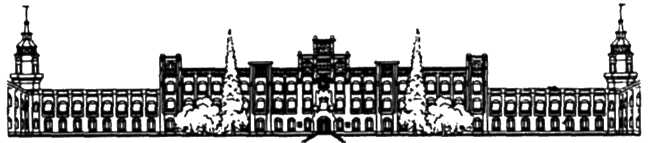
\includegraphics[width=\textwidth]{institute.jpg}}
		}
	\end{frame}\\
	\large
	\centering{
		\vspace{5mm}\\
		Міністерство освіти і науки України \\
		Національний технічний університет України \\
		"Київський політехнічний інститут імені Ігоря Сікорського"\\
		Фізико-технічний інститут
	}
	\vspace{3cm}\\
	\centering{
		{\Huge\textbf{Операційні системи} \\ \vspace{0.15cm}}
		{\huge Лабораторна №9}
	}
	
	\vspace{8cm}
	\Large
	\begin{flushright}
		Виконав:\\
		Студент групи ФБ-82\\
		\textbf{Козачок Вячеслав}\\
		Перевірив: \\
		Кіреєнко О.В.
	\end{flushright}
	\vfill
	
	\centering{Київ - 2020}
	
\end{titlepage}

\subsection{Code}
\begin{lstlisting}[language=C++]
#include <iostream>
#include <pthread.h>
#include <queue>
#include <semaphore.h>
#include <time.h>
#include <unistd.h>

struct thread_info 
{
    int thread_number;
    char * name;
    pthread_t * thread;
};

std::queue<thread_info*> on_board;
std::queue<thread_info*> to_cancel;

sem_t busy_places, boarding, disembarkation;

int paratroopers_on_board = 0;
int marines_on_board = 0;
int max_places;
int handled_soldiers = 0;

void trip()
{
    printf("\n");
    for(int i = 0; i < 3; i++)
    {
        printf("%16s\n", "Ferry in trip!");
        sleep(1);
    }
    printf("\n");

    // Allow troops leave the ferry
    sem_post(&disembarkation);
}

void get_on_board(thread_info * info)
{
    sem_wait(&boarding);
    if(info->name == "Marine")
    {
        if((marines_on_board == max_places/2 && paratroopers_on_board != 0) || (paratroopers_on_board > max_places/2))
        {
            printf("%12s %d canceled ", info->name, info->thread_number);
            to_cancel.push(info);
        } 
        else
        {
            printf("%12s %d boarded  ", info->name, info->thread_number);
            on_board.push(info);
            marines_on_board++;
        }
    }
    else if (info->name == "Paratrooper")
    {
        if((paratroopers_on_board == max_places/2 && marines_on_board != 0) || (marines_on_board > max_places/2))
        {
            printf("%12s %d canceled ", info->name, info->thread_number);
            to_cancel.push(info);
        }        
        else
        {
            printf("%12s %d boarded  ", info->name, info->thread_number);
            on_board.push(info);
            paratroopers_on_board++;
        }
    }

    printf("< Current Time: %d \n", time(0));
    handled_soldiers++;
    sleep(1);
    sem_post(&boarding);
}

void get_out_of_board(thread_info * info)
{
    sem_wait(&disembarkation);
    printf("%12s %d disembarked. < Current time: %d\n", info->name, info->thread_number, time(0));
    sleep(1);
    sem_post(&disembarkation);
}

void clear_ferry()
{
    while(on_board.size() != 0)
    {
        // printf("Waiting clear\n");
        pthread_join(*(on_board.front()->thread), NULL);
        on_board.pop();
    }
}

void cancel_threads()
{
    while(to_cancel.size() != 0)
    {
        pthread_cancel(*(to_cancel.front()->thread));
        to_cancel.pop();
    }
}


void * thread_work(void * param)
{
    thread_info * info = (thread_info*)param;
    sleep(rand() % 3 + 1);
        
    get_on_board(info);
    get_out_of_board(info);
    pthread_exit(NULL);
}

int main(int argv, char * argc[])
{
    std::cout << "Enter N: ";
    int n;
    std::cin >> n;
    if(std::cin.fail())
    {
        std::cout << "Exiting ...\n";
        return 1;
    }

    srand(time(0));
    max_places = n * 2;
    printf("\n%16s\n", "INFORMATION");
    printf("%16s: %d\n", "Available places", max_places);
    printf("%16s: %d\n", "Paratroopers", max_places);
    printf("%16s: %d\n", "Marins", max_places);
    printf("%20s\n", "------------");    
    
    // Semaphores
    sem_init(&boarding, 0, 1);
    sem_init(&disembarkation, 0, 0);

    // Soldiers
    pthread_t * marine = new pthread_t[max_places];
    pthread_t * paratrooper = new pthread_t[max_places];

    int counter = 0;
    thread_info * info;
    for(int i = 0; i < max_places; i++)
    {
        // Creating marine
        info = new thread_info;
        info->thread_number = counter;
        info->thread = &marine[i];
        info->name = "Marine";
        pthread_create(&marine[i], NULL, thread_work, (void*)info);

        // Creating paratrooper
        info = new thread_info;
        info->thread_number = counter;
        info->thread = &paratrooper[i];
        info->name = "Paratrooper";
        pthread_create(&paratrooper[i], NULL, thread_work, ((void*)info));
        counter++;
    }

    // wait till all soldiers is canceled or boarded
    while(handled_soldiers != max_places*2)
    {
        sleep(1);
        continue;
    }

    // remove soldiers that could not board ferry
    printf("\nCleaning all threads troops that are not in ferry\n");
    cancel_threads(); 
    
    trip();

    // clear ferry on another side
    printf("Eject all troops on coast\n\n");
    clear_ferry();
    
    return 0;
}
\end{lstlisting}

\newpage
\subsection*{Output}
\subsubsection*{N = 2}
\begin{lstlisting}[language=BASH]
Enter N: 2

     INFORMATION
Available places: 4
    Paratroopers: 4
          Marins: 4
        ------------
 Paratrooper 0 boarded  < Current Time: 1588159550 
 Paratrooper 2 boarded  < Current Time: 1588159551 
      Marine 0 boarded  < Current Time: 1588159552 
 Paratrooper 1 canceled < Current Time: 1588159553 
      Marine 2 boarded  < Current Time: 1588159554 
      Marine 3 canceled < Current Time: 1588159555 
 Paratrooper 3 canceled < Current Time: 1588159556 
      Marine 1 canceled < Current Time: 1588159557 

Cleaning all threads troops that are not in ferry

  Ferry in trip!
  Ferry in trip!
  Ferry in trip!

Eject all troops on coast

 Paratrooper 0 disembarked. < Current time: 1588159561
 Paratrooper 2 disembarked. < Current time: 1588159562
      Marine 0 disembarked. < Current time: 1588159563
      Marine 2 disembarked. < Current time: 1588159564
\end{lstlisting}

\subsubsection*{N = 3}
\begin{lstlisting}[language=BASH]
\end{lstlisting}

\subsubsection*{N = 5}
\begin{lstlisting}[language=BASH]
Enter N: 5

     INFORMATION
Available places: 10
    Paratroopers: 10
          Marins: 10
        ------------
      Marine 1 boarded  < Current Time: 1588159802 
 Paratrooper 3 boarded  < Current Time: 1588159803 
      Marine 4 boarded  < Current Time: 1588159804 
 Paratrooper 4 boarded  < Current Time: 1588159805 
 Paratrooper 7 boarded  < Current Time: 1588159806 
      Marine 9 boarded  < Current Time: 1588159807 
      Marine 0 boarded  < Current Time: 1588159808 
 Paratrooper 0 boarded  < Current Time: 1588159809 
 Paratrooper 2 boarded  < Current Time: 1588159810 
      Marine 3 boarded  < Current Time: 1588159811 
      Marine 2 canceled < Current Time: 1588159812 
      Marine 5 canceled < Current Time: 1588159813 
 Paratrooper 5 canceled < Current Time: 1588159814 
      Marine 7 canceled < Current Time: 1588159815 
 Paratrooper 8 canceled < Current Time: 1588159816 
 Paratrooper 1 canceled < Current Time: 1588159817 
      Marine 6 canceled < Current Time: 1588159818 
 Paratrooper 6 canceled < Current Time: 1588159819 
      Marine 8 canceled < Current Time: 1588159820 
 Paratrooper 9 canceled < Current Time: 1588159821 

Cleaning all threads troops that are not in ferry

  Ferry in trip!
  Ferry in trip!
  Ferry in trip!

Eject all troops on coast

      Marine 1 disembarked. < Current time: 1588159825
 Paratrooper 3 disembarked. < Current time: 1588159826
      Marine 4 disembarked. < Current time: 1588159827
 Paratrooper 4 disembarked. < Current time: 1588159828
 Paratrooper 7 disembarked. < Current time: 1588159829
      Marine 9 disembarked. < Current time: 1588159830
      Marine 0 disembarked. < Current time: 1588159831
 Paratrooper 0 disembarked. < Current time: 1588159832
 Paratrooper 2 disembarked. < Current time: 1588159833
      Marine 3 disembarked. < Current time: 1588159834

\end{lstlisting}
\begin{lstlisting}[language=BASH]
\end{lstlisting}
\begin{lstlisting}[language=BASH]
\end{lstlisting}

\end{document}